\documentclass[12pt, a4paper]{article}
\usepackage[english, croatian]{babel}
\usepackage{authblk}
\usepackage{listings}

\usepackage{amsmath}
\usepackage{amssymb}
\usepackage{commath}
\usepackage{graphicx}
\usepackage{multicol}
\usepackage{amsfonts}

\usepackage{xcolor}
\usepackage{float}
\usepackage{graphicx}
\usepackage{subcaption}
\usepackage{mwe}
\usepackage{float}
\usepackage{booktabs}
\usepackage{siunitx}
\usepackage[%
colorlinks=true,
pdfborder={0 0 0},
linkcolor=red
]{hyperref}

\newcommand{\R}{$ {\rm I\!R}$}
\definecolor{tb-blue}{HTML}{0077bb}
\definecolor{tb-red}{HTML}{cc3311}

\begin{document}
\date{}
\title{Redukovano GAN obučavanje}
\author{Kosta Grujčić \hspace{25pt} Momčilo Knežević}
\affil{Matematički fakultet}
\maketitle

\begin{abstract}
Generativne suparničke mreže su postale veoma popularan generativan model naročito u oblasti računarskog vida. Nastale su mnogobrojne arhitekture, posebno dizajnirane za različite domene primene. Problem sa ovom vrstom modela je otežana konvergencija, izražena osetljivost na hiperparametre i potreba za velikim skupom podataka za obučavanje. Odlučili smo da proverimo ovu tezu obučavajući DCGAN model nad redukovanim CelebA skupom podataka uvodeći dodatne uslove koji pomažu boljoj konvergenciji.
\end{abstract}

\section{Uvod}
Generativne suparničke mreže (GAN) \cite{GAN-2014} uživaju veliku popularnost kao generativni modeli. Nalaze uspešnu primenu u različitim domenima. Dizajnirane su mnogobrojne arhitekture poput \cite{DCGAN-2016}, \cite{WGAN-2017}, \cite{CGAN-2014}, \cite{StyleGAN-2018}, \cite{StyleGAN2-2019}. Zajednička osobina većine GAN arhitektura je otežana konvergencija usled neograničenog gradijenta, te se nastoji uvođenju restrikcija \cite{Lipschitz-2017}. Usled navedenog problema, potrebno je vršiti iscrpnu pretragu hiperparametara i koristiti veliki skup podataka za obučavanje.

Da bi ispitali u kojoj je meri ovo izraženo, izmenićemo poznatu DCGAN arhitekturu uvodeći spektralnu normalizaciju \cite{SN-2018} i redukujući skup podataka CelebA \cite{CelebA-2015}. Obučavanje kvantifikujemo poznatim metrikama IS (eng. \textit{inception score}) \cite{IS-2016} i FID (eng. \textit{Fréchet Inception distance}) \cite{FID-2017}. Očekujemo da je moguče dobiti reprezentativno obučen model upotrebom spektralne normalizacije na redukovanom skupu podataka.

\section{Pređašnji rad}
U ovom poglavlju ćemo opisati princip rada GAN-ova, GAN arhitekturu koju koristimo i metrika kojima ćemo kvantifikovati obučenost modela.

\subsection{Generativne suparničke mreže}
	Prvo dajemo neformalnu ideju. Osnovni cilj je naučiti raspodelu podataka tako da je moguće vršiti uzorkovanje, čime se dobija mogućnost generisanja podataka koji zapravo ne postoje. GAN arhitektura podrazumeva upotrebu dva modela. Prvi je zadužen za učenje pomenute raspodele, dok drugi treba da razlikuje stvarne i generisane podatke. Suparničkim učenjem ova dva modela se stvarna raspodela podataka sve bolje aproksimira.
	
	Neka je $\mathcal{X}\subset \R^{c \times d \times d}$ prostor $c$-kanalnih slika dimenzija $d\times d$. Bilo koji skup slika možemo predstaviti nekom raspodelom $p_r$ nad $\mathcal{X}$. Skup nad kojim obučavamo model možemo definisati kao prost slučajan uzorak iz raspodele $p_r$. Cilj je naučiti parametrizovanu raspodelu $p_g$ koja aproksimira $p_r$.
	
	GAN se sastoji od \textit{generatora} i \textit{diskriminatora}. Diskriminator posmatramo kao preslikavanje $D: \mathcal{X} \rightarrow [0, 1]$, dok generator kao $G:\mathcal{Z} \rightarrow \mathcal{X}$, gde je $\mathcal{Z}$ latentni prostor. Pomenuti latentni prostor služi za uzorkovanje šuma na osnovu kojeg generator pokušava da generiše elemente raspodele $p_r$. Ako takvo uzorkovanje šuma vršimo iz raspodele $p_z$ definisane nad $\mathcal{Z}$, tada raspodelu $p_g$ možemo definisati kao $G(p_z)$.
	
	Napomenimo da male vrednosti diskriminatora odgovaraju generisanim podacima, dok veće stvarnim. Prema tome, generator nastoji generisanju podataka za koje diskriminator daje vrednosti bliske $1$, dok diskriminator za takve ulaze nastoji da se sve viši približi vrednosti $0$.
	
	Obučavanje diskriminatora i generatora se vrši uporedo, usled čega se može videti kao min-max igra. Takav proces se može formalizovati:
	\begin{equation}
	\min_{G}\max_{D}V(D, G) = \mathbb{E}_{x \sim p_r}[\log D(x)] + \mathbb{E}_{z \sim p_z}[\log(1 - D(G(z)))].
	\label{eq:GANClassic}
	\end{equation}
	
	Primetimo da ne postoji ograničenje za izbor modela $D$ i $G$. Međutim, pretpostavljajući njihovu diferencijabilnost i parametrizovanost, obučavanje se može vršiti propagacijom unazad i time u velikoj meri automatizovati.
	
	U početnim iteracijama obučavanja može doći do zasićenja gradijenata \cite{GAN-2014}. Usled lošeg generatora, diskriminator je u stanju vrlo precizno da razlikuje lažne i prave podatke. S tim u vezi, optimizacija iz formule \ref{eq:GANClassic} se može zapisati u numerički pogodnijem obliku:
	\begin{equation}
	\min_{G}\max_{D}V(D, G) = \mathbb{E}_{x \sim p_r}[\log D(x)] - \mathbb{E}_{z \sim p_z}[\log D(G(z))].
	\label{eq:GAN_BCE}
	\end{equation}

\subsection{DCGAN}
Generativne suparničke mreže ne podrazumevaju nikakav konkretan model ni za generator ni za diskriminator. S tim u vezi, zavisnosti od domena primene se mogu dizajnirati odgovarajući modeli. Kako se CelebA sastoji od slika, to se opredeljujemo za arhitekturu baziranu na konvolutivnim neuronskim mrežama. Koristićemo DCGAN arhitekturu \cite{DCGAN-2016}, pre svega zbog povoljnog vremena obučavanja.

Prvo ćemo objasniti strukturu diskriminatora ove arhitekture. Sastoji se $5$ blokova koji vrše decimaciju prostornih dimenzija ulaznog tenzora za faktor $2$. Svaki blok se sastoji od konvolutivnog sloja praćenog BN slojem \cite{BN-2015}, osim u poslednjem bloku gde ne postoji sloj normalizacije. Aktivaciona funkcija u svakom konvolutivnom sloju je ReLU \cite{ReLU-2010}, osim u poslednjem gde je sigmoid. Konvolutivni slojevi imaju redom $128, 256, 512, 1024, 1$ kanala. Decimacija je postignuta postavljanjem pomeraja konvolutivnog sloja na $2$. Ulazni tenzor je trokanalna RGB slika, koja se prethodno normalizuje sa $\hat{\mu}=0.5$ i $\hat{\sigma}=0.5$.

Generator u odnosu na diskriminator ima inverznu strukturu. Koristi $4$ ekspanziona bloka i transponovane konvolutivne slojeve umesto običnih. Broj kanala u konvolutivnim slojevima je redom $512, 256, 128, 3$. Pre nego što se latentni šum prosledi prvom konvolutivnom sloju, vrši se projektovanje potpuno povezanim slojem u prostor $\R^{1024 \times 4 \times 4}$. Aktivaciona funkcija poslednjeg sloja je hiperbolički tangens.

Funkcija greške je binarna unakrsna entropija. Iz formule \ref{eq:GAN_BCE} se vrlo lako dobija oblik funkcije greške za obe komponente.

\subsection{Lipšic neprekidnost generatora}
Pretpostavimo da je diskriminator $D$ neuronska mreža koja za ulaz $x\in \mathcal{X}$ ima sledeći oblik:
\begin{equation}
f(x, \theta) = \left(\prod^{L}_{i=1} a_{i}(\beta_i + W_{i})\right)(x),
\end{equation}
gde je $\theta = \{W_i\}^{L}_{i=1}$ skup parametara koji se obučavaju, $W_i \in \R^{d_i \times d_{i-1}}$ i $\{a_i\}^{L}_{i=1}$ aktivacione funkcije koje se primenjuju član po član. Napomenimo da $d_0$ predstavlja broj kanala ulaza, dok je $d_L=1$.

Dokazano je \cite{GAN-2014} da za fiksiran generator $G$, optimalan diskriminator ima oblik:
\begin{equation}
D^{\ast}_{G}(x) = \frac{p_r(x)}{p_r(x) + p_g(x)}=\sigma(f^{\ast}(x)),
\end{equation}
gde je $\sigma$ sigmoid, a $f^{\ast}(x) = \log{p_r(x)} - \log{p_g(x)}$. Tada dobijamo:
\begin{equation}
\nabla_x D^{\ast}_{G}(x) \propto \nabla_x f^{\ast}(x)=\frac{1}{p_r(x)}\nabla_x p_r(x)-\frac{1}{p_g(x)}\nabla_x p_g(x).
\label{eq:grad}
\end{equation}
Primetimo da gradijent $\nabla_x f^{\ast}(x)$ nije ograničen. Iz tog razloga dolazi do nepredvidivih oscilacija tokom obučavanja i česte divergencije. Zato je neophodno nametnuti dodatne uslove za $f$. Na osnovu \cite{Lipschitz-2017}, diskriminator obučavamo u prostoru $K$-Lipšic neprekidnih funkcija\footnote{$(\exists K > 0)(\forall x, y \in \mathcal{D}) \norm{f(x) - f(y)} \leq K \cdot \norm{x-y}$}. Tada je gradijent iz formule \ref{eq:grad} ograničen. Formula \ref{eq:GANClassic} postaje:
\begin{equation}
\min_G \max_{\norm{f}_{\operatorname{Lip} \leq K}} V(D, G),
\end{equation}
gde je $\norm{f}_{\operatorname{Lip} \leq K}$ skup svih $K$-Lipšic neprekidnih funkcija u metričkom prostoru $(\mathcal{X}, l_2)$.

Spektralna normalizacija (SN) \cite{SN-2018} se zasniva na uslovu $\norm{W_i}_2=1$. Kako je $\norm{W_i}_2 = \sqrt{\lambda_{\text{max}}(W^{T}_{i} W_i)}$, to je neophodno odrediti najveću sopstvenu vrednost matrice $W^{T}_{i} W_i$. Pomenuti postupak je moguće sprovesti numerički.

U odnosu na standardnu DCGAN implementaciju, u našim eksperimentima je SN korišćena umesto BN i to isključivo kod diskriminatora.

\subsection{IS}
Adekvatno obučen GAN poseduje sigurnost i varijabilnost. To znači da generator može dati svojstvene podatke, kao i da ravnomerno pokriva čitav kombinatorni prostor.

Prepostavimo da svakoj instanci skupa podataka $x$ možemo pridružiti oznaku $y$. Skup podataka takve oznake ne mora da sadrži, ali ih je moguće uvesti dodatnim modelom $\mathcal{M}$ (kao što je Inception \cite{Inception-2014}) koji je treniran kao klasifikacioni model na nekom drugom skupu podataka (kao što je ImageNet \cite{ImageNet-2014}). Zato možemo posmatrati uslovnu raspodelu $p_{\mathcal{M}}(y|x)$. Marginalna raspodela $p_{\mathcal{M}}(y)$ se dobija kao $\int_{x}p_{\mathcal{M}}(y|x)\text{d}p_g(x)$.

Prema tome, $p_g(y|x)$ treba da odgovara Dirakovoj $\delta$ funkciji, a $p_g(y)$ ravnomernoj raspodeli. Konačno, IS definišemo:
\begin{equation}
\operatorname{IS}(p_g) = \exp(\mathbb{E}_{x \sim p_g}[D_{KL}(p_\mathcal{M}(y|x)||p_\mathcal{M}(y))]),
\end{equation}
gde je $D_{KL}$ Kulbek-Lajblerova divergencija.

Ispostavlja se da ova metrika dobro korelira sa ljudskom odlukom \cite{IS-2016}. Međutim, IS ni na koji način ne koristi $p_r$. Takođe, skup podataka nad kojim je $\mathcal{M}$ treniran možda nema ni približno sličnu raspodelu kao $p_r$ usled čega GAN model biva proglašen lošim.

\subsection{FID}
Kao što smo već rekli, ideja obučavanja GAN-a je što bolja aproksimacija $p_r$ raspodelom $p_g$. Ukoliko $p_r$ predstavlja raspodelu podataka iz realnog sveta (poput slika ljudi), tada možemo pretpostaviti ograničenost njenog nosača. U tom slučaju važi:
\begin{equation}
p_r \stackrel{s.s.}{=} p_q \iff (\forall k \in \mathbb{N}) \int_{\mathcal{X}} p_r(x) x^k \text{d}x = \int_{\mathcal{X}} p_g(x) x^k \text{d}x.
\label{eq:probEquality}
\end{equation}
Drugim rečima, jednakost momenata povlači skoro sigurnu jednakost raspodela. U praksi je desnu stranu ekvivalencije \ref{eq:probEquality} skoro nemoguće pokazati. Zato se ona aproksimira za vrednosti do nekog $k$. Mi ćemo aproksimaciju vršiti za $k=2$.

Kako raspodele $p_r$ i $p_g$ nisu eksplicitno poznate, uvodimo operator $\phi$ tako da jednakost $\phi(p_r)$ i $\phi(p_g)$ odgovara jednakosti odgovarajućih raspodela. Kao i kod IS, koristimo Inception model čiji će neki unutrašnji sloj predstavljati operator $\phi$. Inception model obučen nad ImageNet skupu podataka poseduje kvalitetnu aproksimaciju raspodele slika iz stvarnog sveta čiji duboki slojevi poseduju vizuelne karakteristike visokog nivoa. Iz tog razloga, za očekivati je da forsiranjem sličnosti $\phi(p_r)$ i $\phi(p_g)$ postižemo sličnost $p_r$ i $p_g$.

Međutim, raspodele $\phi(p_r)$ i $\phi(p_g)$ takođe nisu eksplicitno poznate. Poznato je da za fiksirane momente prva dva reda normalna raspodela ima maksimalnu entropiju. Zato pretpostavljamo: $\phi(p_r) = \mathcal{N}(\mu_r, \Sigma_r)$ i $\phi(p_g) = \mathcal{N}(\mu_g, \Sigma_g).$ Razliku ovih raspodela merimo Frešeovim rastojanjem:
\begin{equation}
F(\phi(p_r), \phi(p_g)) = \norm{\mu_r - \mu_g} + \text{tr}\left(\Sigma_r + \Sigma_g - 2(\Sigma_r \Sigma_g)^{1/2}\right),
\end{equation}
gde je $\text{tr}$ operator traga matrice.

Konačno, definišemo $\operatorname{FID}(p_r, p_g)$ kao $F(\phi(p_r), \phi(p_g))$ \cite{FID-2017}. Primetimo da za razliku od IS, FID koristi $p_r$.

\section{Eksperimenti}
Koristili smo dve arhitekture, DCGAN \cite{DCGAN-2016} i SN-DCGAN \cite{SN-2018}. Za obučavanje je korišćena \texttt{Python} biblioteka \texttt{PyTorch} \cite{PyTorch-2019}. Svi eksperimenti su vršeni upotrebom servisa Google Colaboratory na kom smo imali pristup Nvidia T4 i Nvidia P100 grafičkim procesorima. Implementacija se na nalazi na GitHub repozitorijumu\footnote{https://github.com/4eyes4u/RI-GAN}.

Skup CelebA ima $202599$ instanci. U našim eksperimentima je korišćeno $89931$, što predstavlja redukciju od oko $55\%$. Ovaj skup podataka se sastoji od slika lica poznatih ličnosti različite boje kože, odeće i dodatnih karakteristika poput naočara, nakita ili šminke.

Sve slike su rezolucije $64 \times 64$. Obučavanje je vršeno u trajanju od 30 epoha. Korišćen je Adam optimizator za generator i diskriminator. U slučaju spektralne normalizacije, broj iteracija potrebnih za aproksimiranje najveće sopstvene vrednosti ($k$) je iz skupa $\{1, 2, 3\}$. Svi ostali parametri su korišćeni u skladu sa \cite{DCGAN-2016}. Svi modeli su obučavani po $3$ puta za svaku konfiguraciju i uzeta je srednja vrednost.

Dužina trajanja epohe je redom $14$ i $5$ minuta na T4 i P100.

U tablici \ref{table:is-fid} su prikazane vrednosti IS i FID metrika za sve konfiguracije.

\begin{table}[h]
	\centering
	\begin{tabular}{SSS} \toprule
		{model} & {IS} & {FID} \\ \midrule
		{DCGAN} & \textbf{1.93}  & 27.72 \\ 
		{SN(1)-DCGAN} & 1.84 & 24.61 \\
		{SN(2)-DCGAN} & 1.80 & 24.54 \\
		{SN(3)-DCGAN} & 1.80 & \textbf{23.39} \\ \bottomrule
	\end{tabular}
	\caption{Poređenje metrika obučenih modela. SN($k$)-DCGAN označava SN-DCGAN sa vrednošću parametra $k$.}
	\label{table:is-fid}
\end{table}

%\subsection{Uticaj spektralne normalizacije}
%U ovom eksperimentu utvđujemo da li i koliko spektralna normalizacija poboljšava generator.
%
%Pri istim uslovima poredimo rezultate modela sa i bez spektralne normalizacije. Obučavanje vršimo za sve dopustive vrednosti parametra $k$.

%\subsection{Uticaj veličine skupa za obučavanje}
%U ovom eksperimentu utvrđujemo da li je inicijalni skup podataka moguće redukovati, a postići uporediv kvalitet modela.
%
%Iz celog skupa podataka, ravnomernom raspodelom uzorkujemo $30\%$, $50\%$, $70\%$ i $90\%$ podataka.

%\subsection{Merenje preprilagođenosti}
%U ovom eksperimentu utvrđujemo da li je došlo do preprilagođavanja modela i u kojoj meri.
%
%Skup podataka $S$ podelimo na dva podskupa $S_{train}$ i $S_{val}$. Metriku koju koristimo za ocenu kvaliteta obučenosti modela označimo sa $d$. Skup slika generisanih od strane generatora označimo sa $S_g$. Model obučavamo nad $S_{train}$, dok se $S_{val}$ ne koristi tokom obučavanja. Ukoliko model dobro generalizuje, tada $\frac{d(S_{train}, S_g)}{d(S_{val}, S_g)} \rightarrow 1$, dok u suprotnom $\frac{d(S_{train}, S_g)}{d(S_{val}, S_g)} \rightarrow 0$. Skup $S$ delimo u razmeri $30:70$ i $10:90$.

\section{Rezultati}
Na osnovu tablice \ref{table:is-fid} primećujemo sledeće:
\begin{itemize}
	\item Modeli su praktično identični prema IS metrici. To možemo objasniti izraženom robusnošću Inception modela kao i glavnim nedostakom IS metrike -- ne uzima u obzir stvarne podatke. Za očekivati je da su $\mathcal{M}$ raspodele svih modela veoma slične jer raspodele $p_g$ u odnosu na $\mathcal{M}$ predstavljaju slične raspodele ljudskih lica.
	
	\item Modeli se razlikuju prema FID metrici. Budući da FID metrika koristi $p_r$ za očekivati je da postoji razlika u kvalitetu modela ukoliko spektralna normalizacija ima uticaj na obučavanje. Kako je na osnovu pojedinačnih primera jasno da to jeste slučaj, FID metrika to i potvrđuje. SN($3$)-DCGAN očito jeste najbolji model, što svakako i treba da bude imajući u vidu da vrši najprecizniju aproksimaciju $l_2$ norme.
	
	\item Na slici \ref{fig:comparison} su istaknuti nasumično odabrani primeri iz odgovarajućih $p_g$ raspodela. Primetan je definitivan uticaj spektralne normalizacije u obučavanju što je u saglasnosti sa  FID metrikom. Slike koje DCGAN generiše su primetno isprane i lošije od ostalih modela. SN($k$)-DCGAN modeli uglavnom generišu kvalitetne slike, uz poneke izutetke u vidu neprirodnih boja ili distorzije lica.
\end{itemize}

\begin{figure}[H]
	\centering
	\begin{subfigure}[b]{0.475\textwidth}
		\centering
		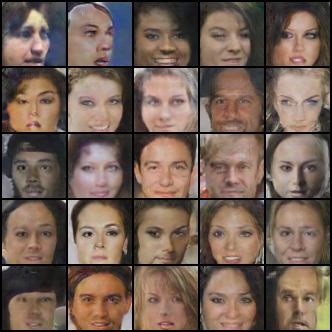
\includegraphics[width=\textwidth]{DCGAN.png}
		\caption[Network2]%
		{{\small DCGAN}}    
		\label{fig:mean and std of net14}
	\end{subfigure}
	\hfill
	\begin{subfigure}[b]{0.475\textwidth}  
		\centering 
		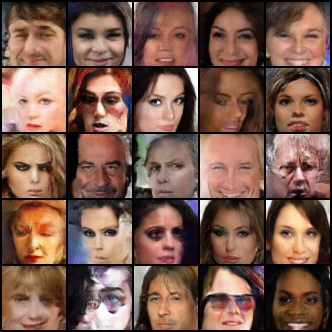
\includegraphics[width=\textwidth]{SN(1)-DCGAN.png}
		\caption[]%
		{{\small SN(1)-DCGAN}}    
		\label{fig:mean and std of net24}
	\end{subfigure}
	\vskip\baselineskip
	\begin{subfigure}[b]{0.475\textwidth}   
		\centering 
		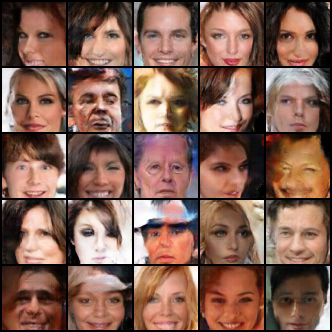
\includegraphics[width=\textwidth]{SN(2)-DCGAN.png}
		\caption[]%
		{{\small SN(2)-DCGAN}}    
		\label{fig:mean and std of net34}
	\end{subfigure}
	\hfill
	\begin{subfigure}[b]{0.475\textwidth}   
		\centering 
		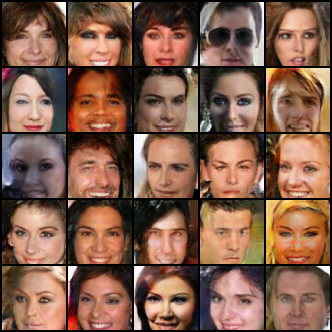
\includegraphics[width=\textwidth]{SN(3)-DCGAN.png}
		\caption[]%
		{{\small SN(3)-DCGAN}}    
		\label{fig:mean and std of net44}
	\end{subfigure}
	\caption[]
	{\small Poređenje rezultata nakon obučavanja. SN($k$)-DCGAN označava SN-DCGAN sa vrednošću parametra $k$.} 
	\label{fig:comparison}
\end{figure}

\section{Zaključak}
Na osnovu prikazanih rezultata uticaj spektralne normalizacije je neupitan. Takođe, pokazuje se da je moguće dobiti konkurentne modele sa redukovanim skupom za obučavanje što i jeste bio cilj ovog rada.

Interesantno je proveriti uticaj spektralne normalizacije na preprilagođenost modela. Mišljenja smo da spektralna normalizacija ne dovodi do preprilagođavanja jer isključivo utiče na glatkoću mnogostrukosti funkcije greške.

\section*{Dodatak A}
Ovde prikazujemo nekoliko primera interpolacije upotrebom SN($3$)-DCGAN modela. Slike su interpolirane upotrebom linearne interpolacije u 16 koraka. Prikazano je ukupno $14$ interpolacija od kojih svaka zauzima $2$ reda. Slike su izvorno rezolucije $64 \times 64$, ali su ovde prikazane u rezoluciji $128 \times 128$ kao rezultat bilinearne interpolacije.

\centerline{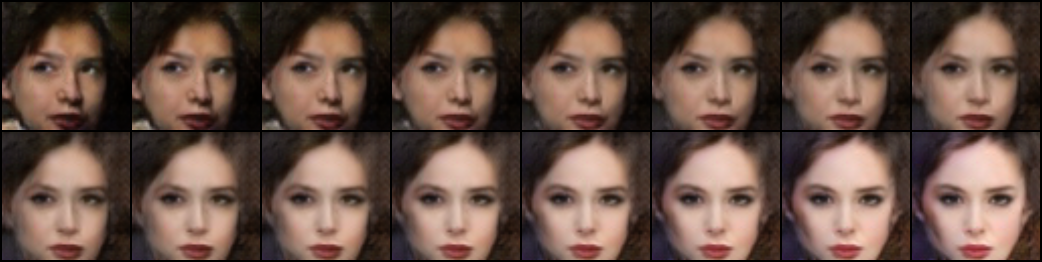
\includegraphics[width=0.9\paperwidth]{inter14.png}}
\centerline{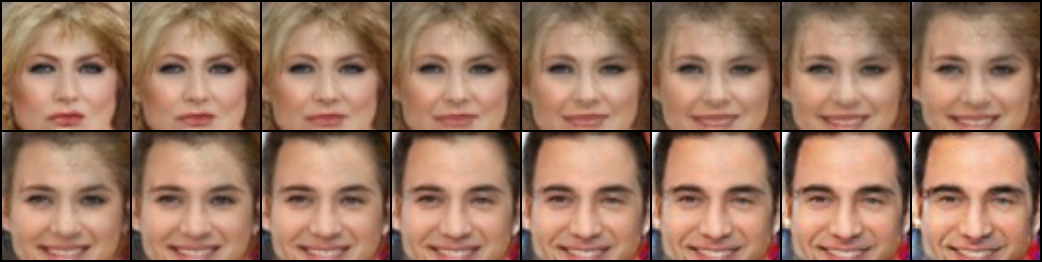
\includegraphics[width=0.9\paperwidth]{inter20.png}}
\centerline{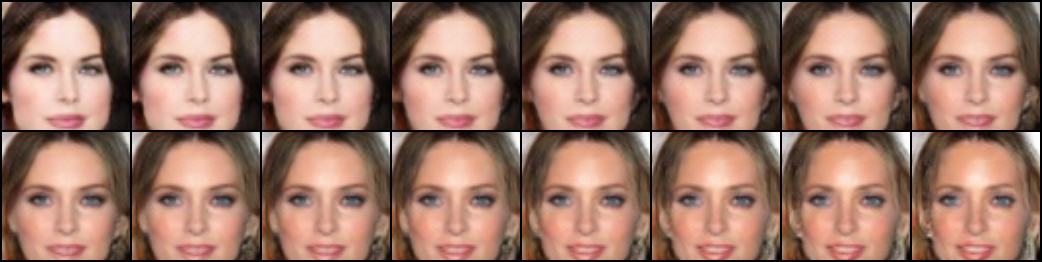
\includegraphics[width=0.9\paperwidth]{inter25.png}}
\centerline{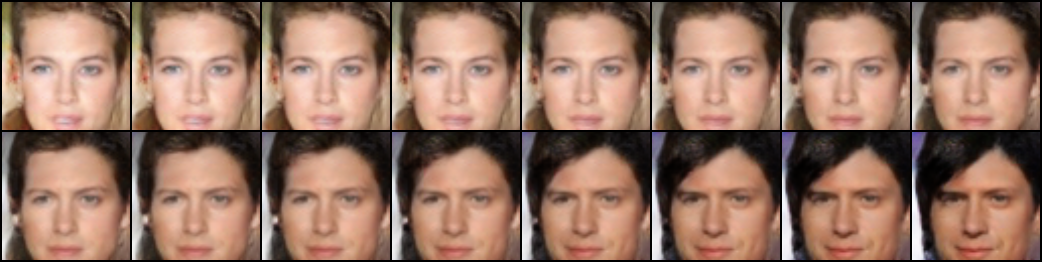
\includegraphics[width=0.9\paperwidth]{inter29.png}}
\centerline{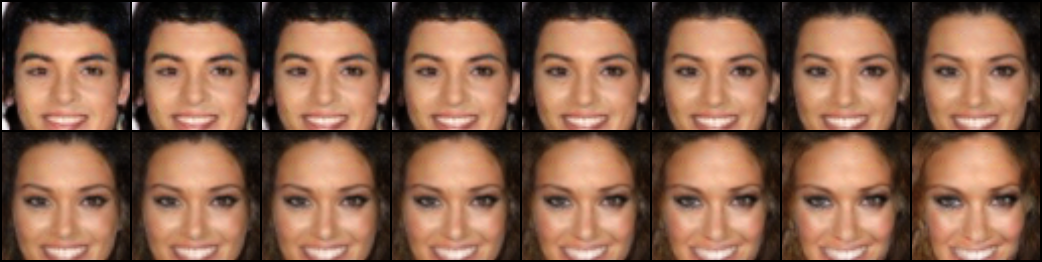
\includegraphics[width=0.9\paperwidth]{inter53.png}}
\centerline{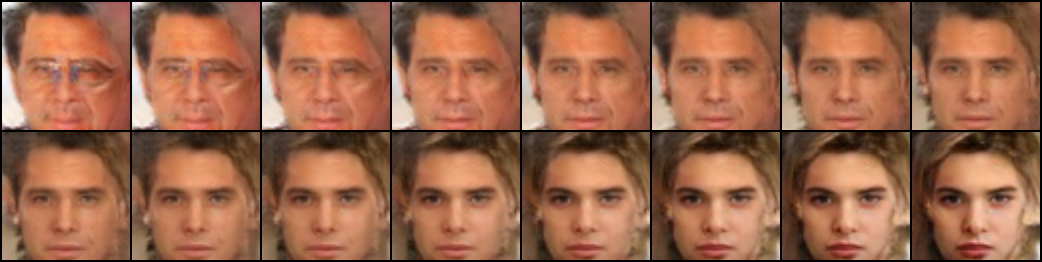
\includegraphics[width=0.9\paperwidth]{inter63.png}}
\centerline{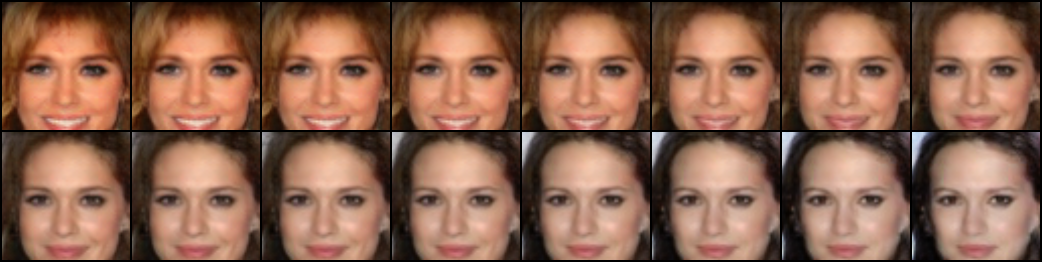
\includegraphics[width=0.9\paperwidth]{inter66.png}}
\centerline{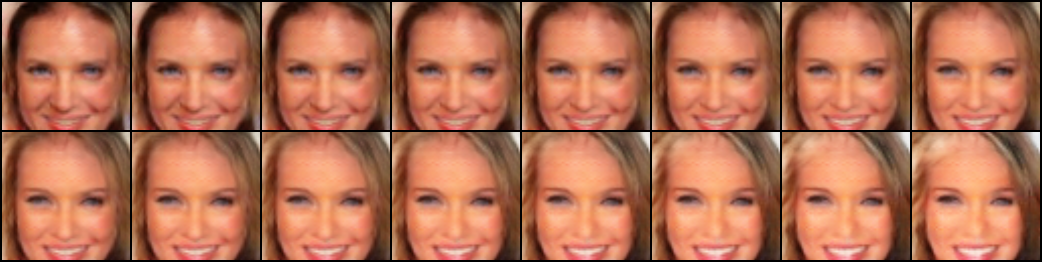
\includegraphics[width=0.9\paperwidth]{inter115.png}}
\centerline{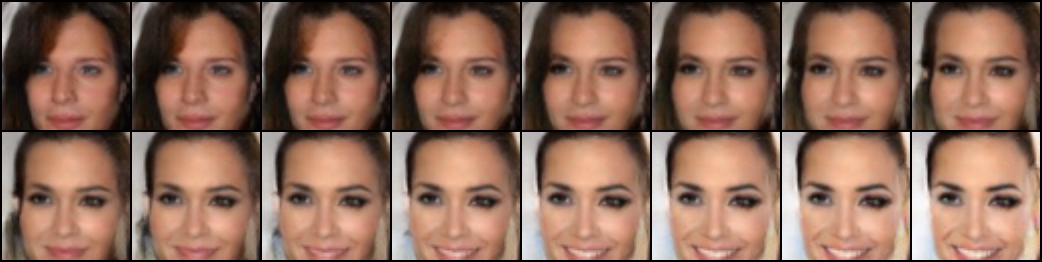
\includegraphics[width=0.9\paperwidth]{inter127.png}}
\centerline{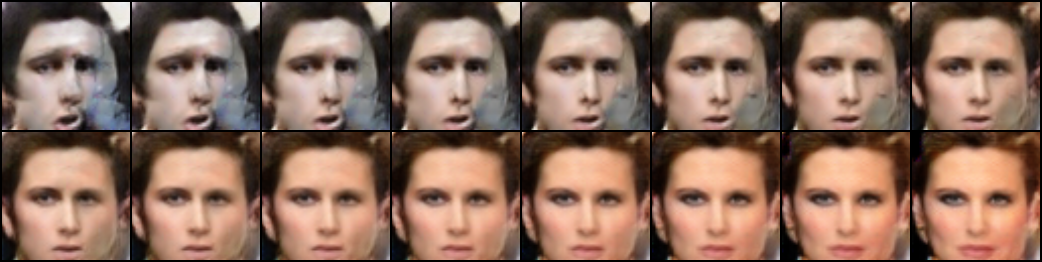
\includegraphics[width=0.9\paperwidth]{inter232.png}}
\centerline{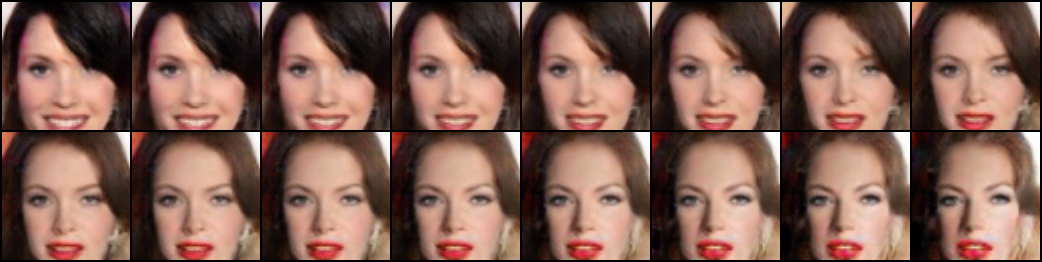
\includegraphics[width=0.9\paperwidth]{inter292.png}}
\centerline{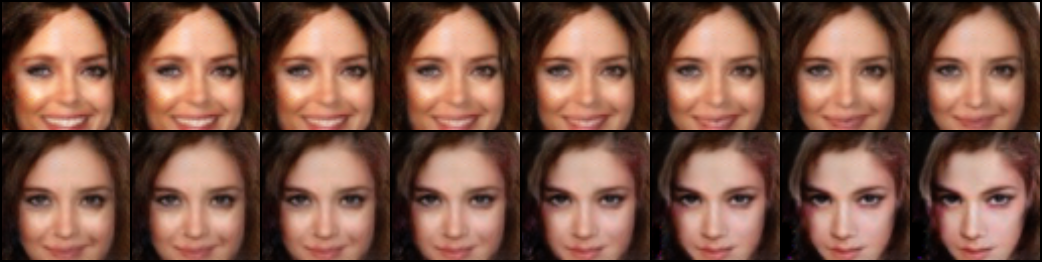
\includegraphics[width=0.9\paperwidth]{inter341.png}}
\centerline{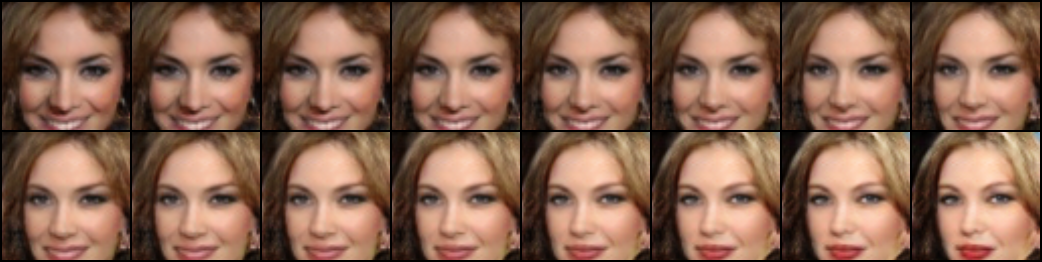
\includegraphics[width=0.9\paperwidth]{inter443.png}}
\centerline{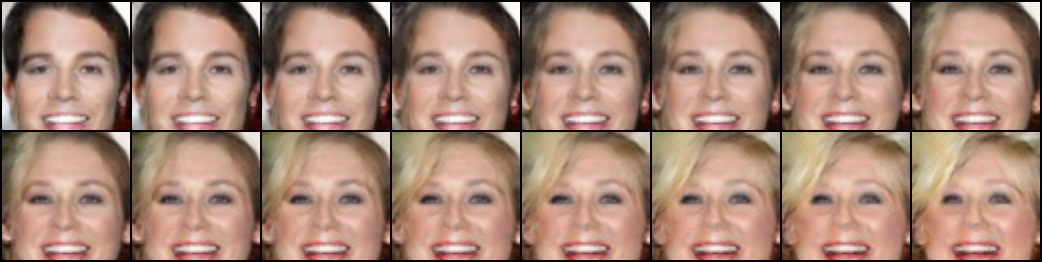
\includegraphics[width=0.9\paperwidth]{inter486.png}}

\section*{Dodatak B}
Ovde prikazujemo funkciju greške svih modela tokom obučavanja. Da bi prikazali usrednjenu funkciju greške, grafici su čuvani u \texttt{TensorBoard} formatu i ufinjeni faktorom $0.85$. Možemo primetiti sledeće:
\begin{itemize}
	\item U slučaju DCGAN modela brzo dolazi do stagnacije diskriminatora, čija je funkcija greške približno $0$. Tada gradijent iz \ref{eq:grad} praktično ne postoji i generator nije u stanju da napreduje.
	\item Funkcija greške diskriminatora u slučaju SN($k$)-DCGAN modela evidentno opada tokom treninga, ali na asimptotski povoljniji način. Usled takvog ponašanja diskriminatora gradijent iz \ref{eq:grad} neće ni nestati ni eksplodirati te se generator daleko bolja obučava.
	\item Bez obzira da li se spektralna normalizacija upotrebljava ili ne, primetan je značajan šum u obučavanju.
\end{itemize}

\begin{figure}[H]
	\centerline{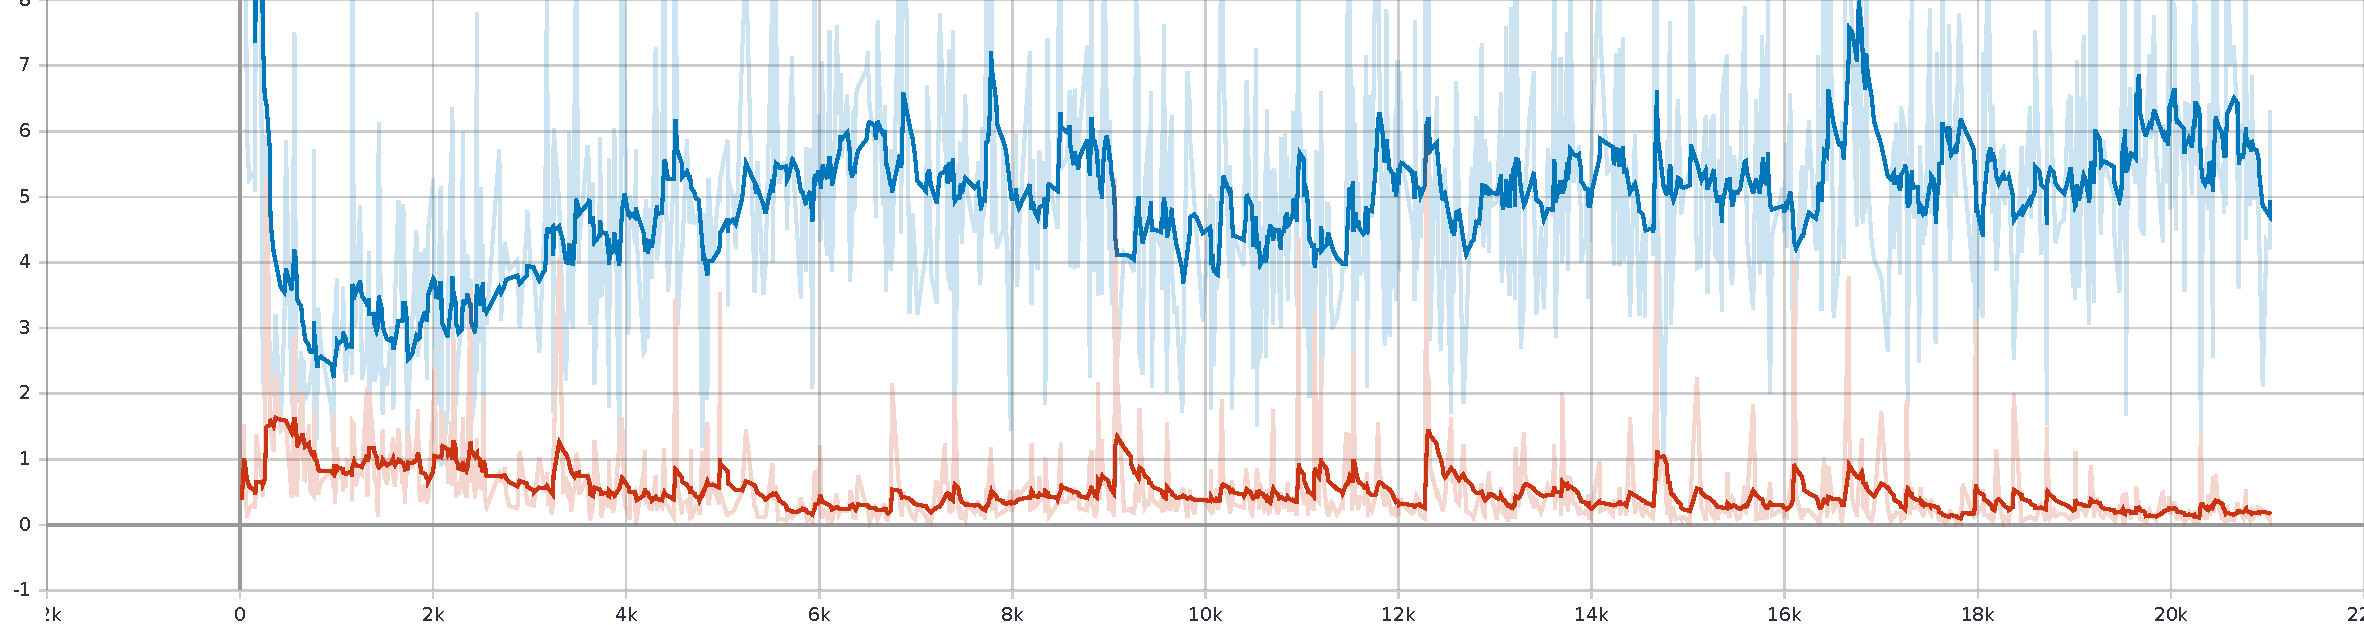
\includegraphics[width=1.5\linewidth]{DCGAN_loss.pdf}}
	\caption{Funkcija greške DCGAN modela. \textcolor{tb-blue}{Generator} i  \textcolor{tb-red}{Diskriminator}.}
	\label{fig:DCGAN_loss}
\end{figure}
\begin{figure}[H]
	\centerline{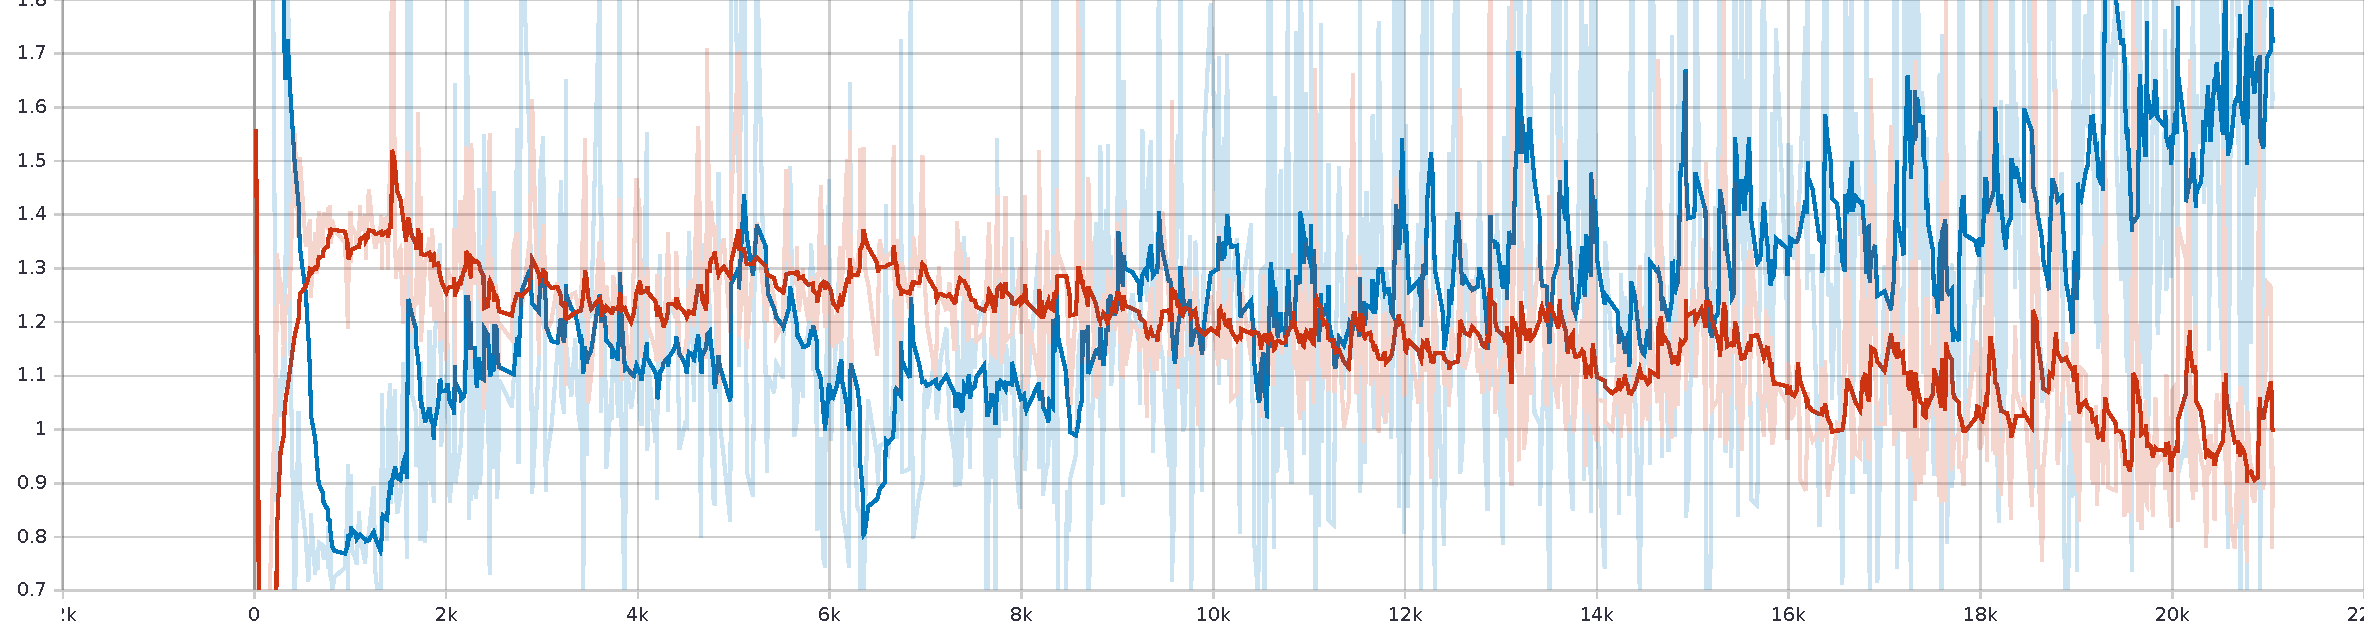
\includegraphics[width=1.5\linewidth]{SN(1)-DCGAN_loss.pdf}}
	\caption{Funkcija greške SN(1)-DCGAN modela. \textcolor{tb-blue}{Generator} i  \textcolor{tb-red}{Diskriminator}.}
	\label{fig:SN(1)-DCGAN_loss}
\end{figure}
\begin{figure}[H]
	\centerline{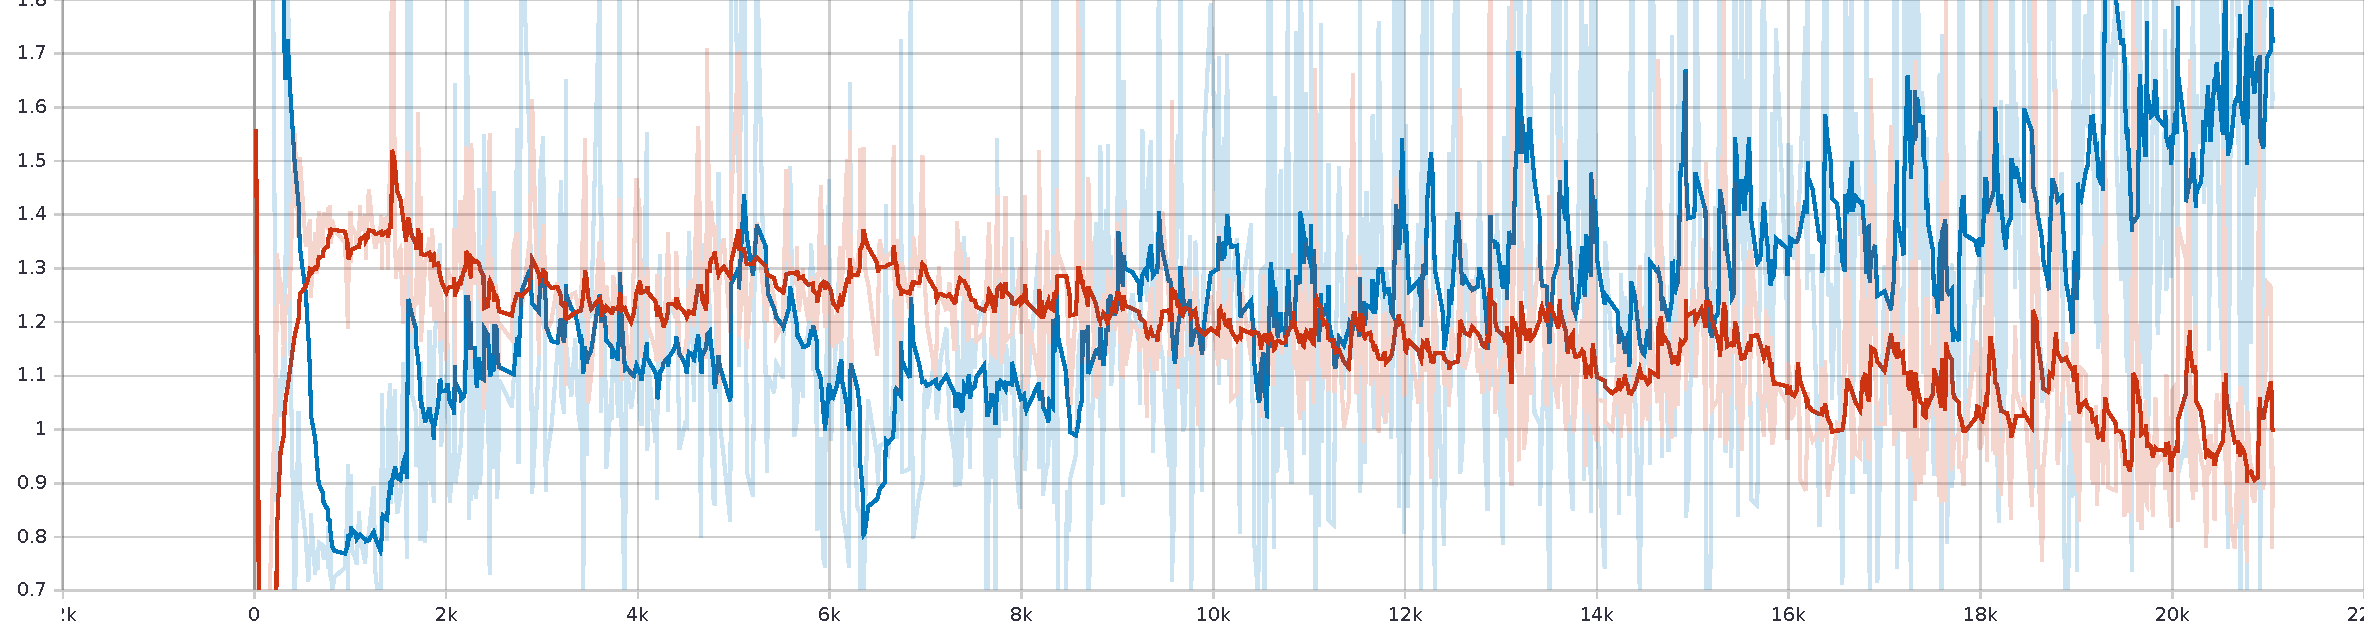
\includegraphics[width=1.5\linewidth]{SN(2)-DCGAN_loss.pdf}}
	\caption{Funkcija greške SN(2)-DCGAN modela. \textcolor{tb-blue}{Generator} i  \textcolor{tb-red}{Diskriminator}.}
	\label{fig:SN(2)-DCGAN_loss}
\end{figure}
\begin{figure}[H]
	\centerline{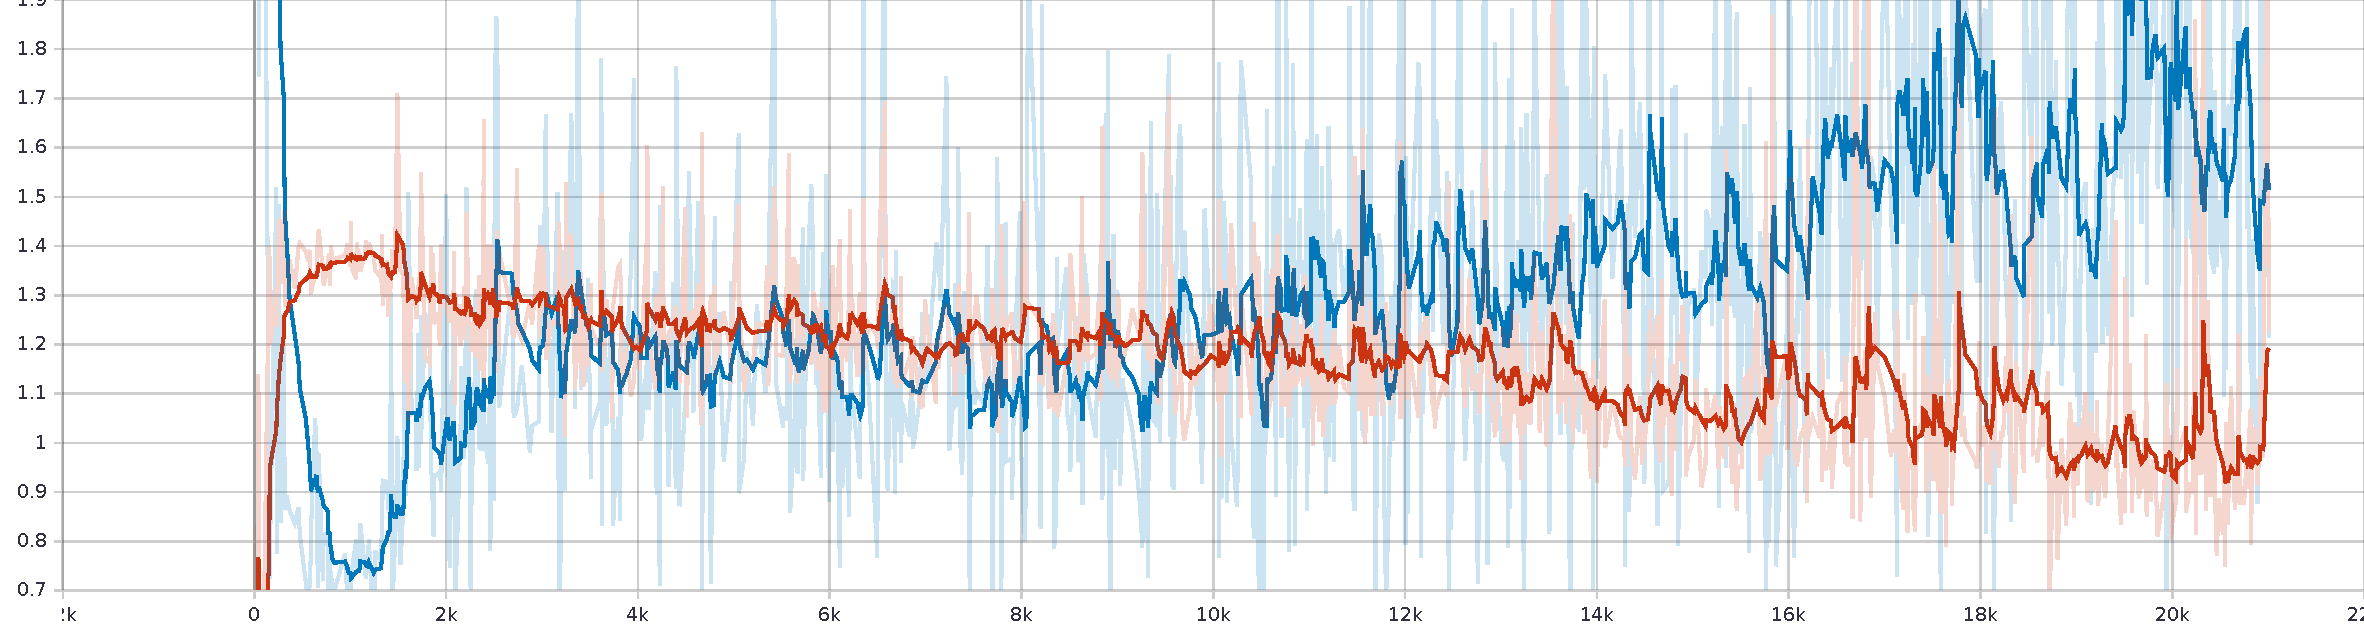
\includegraphics[width=1.5\linewidth]{SN(3)-DCGAN_loss.pdf}}
	\caption{Funkcija greške SN(3)-DCGAN modela. \textcolor{tb-blue}{Generator} i  \textcolor{tb-red}{Diskriminator}.}
	\label{fig:SN(3)-DCGAN_loss}
\end{figure}
%\centerline{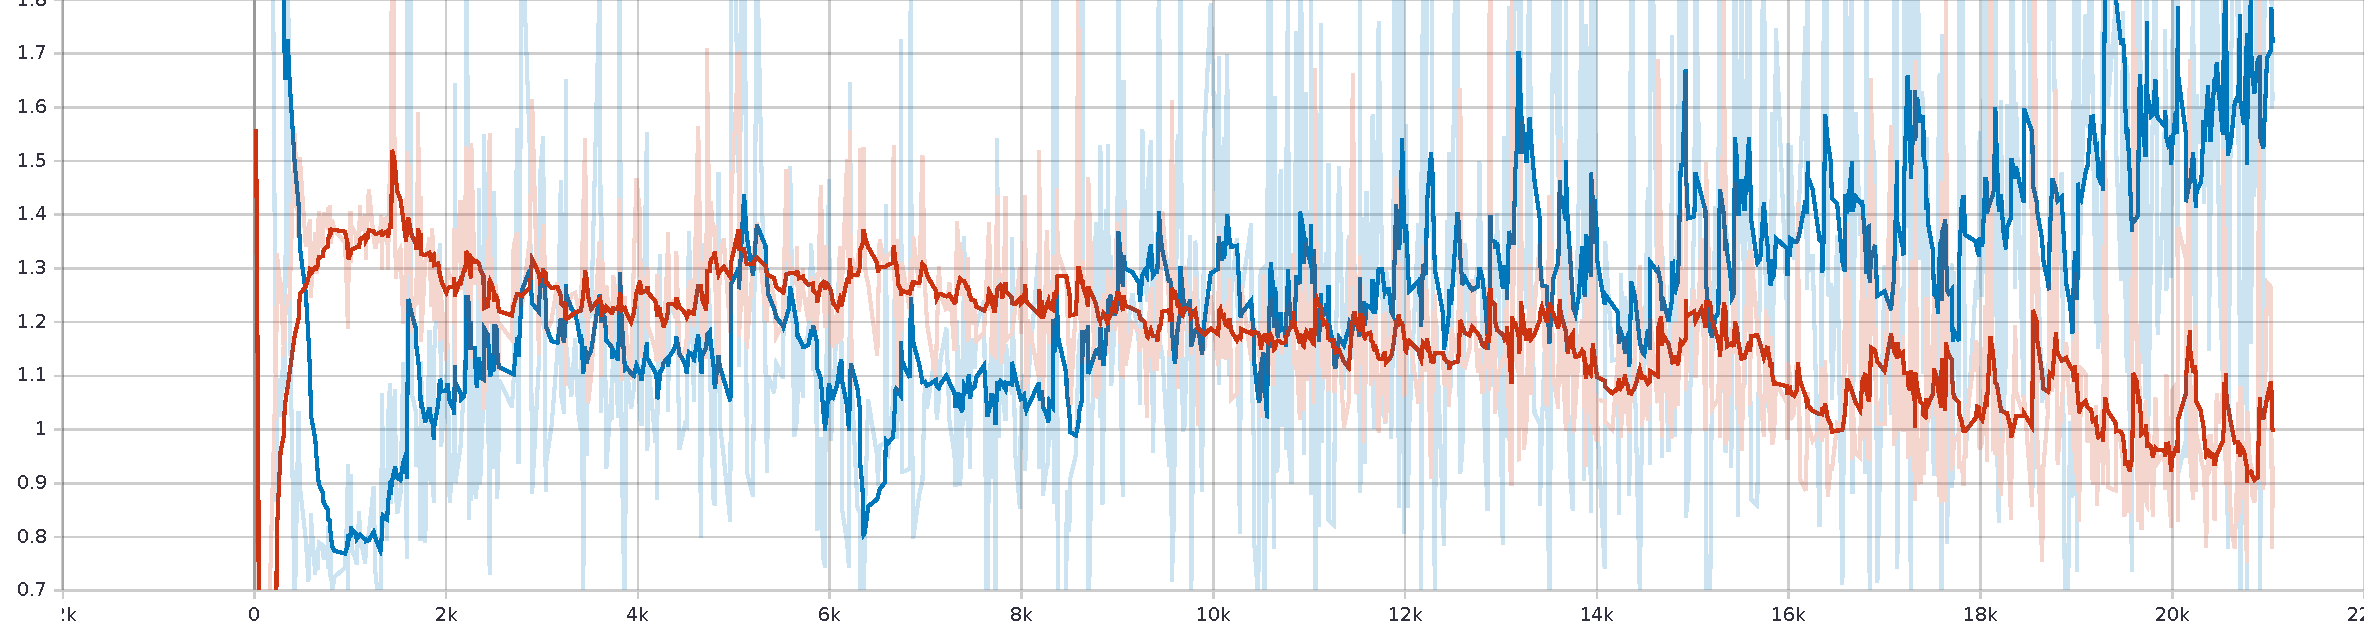
\includegraphics[width=1.5\linewidth]{SN(1)-DCGAN_loss.pdf}}
%\centerline{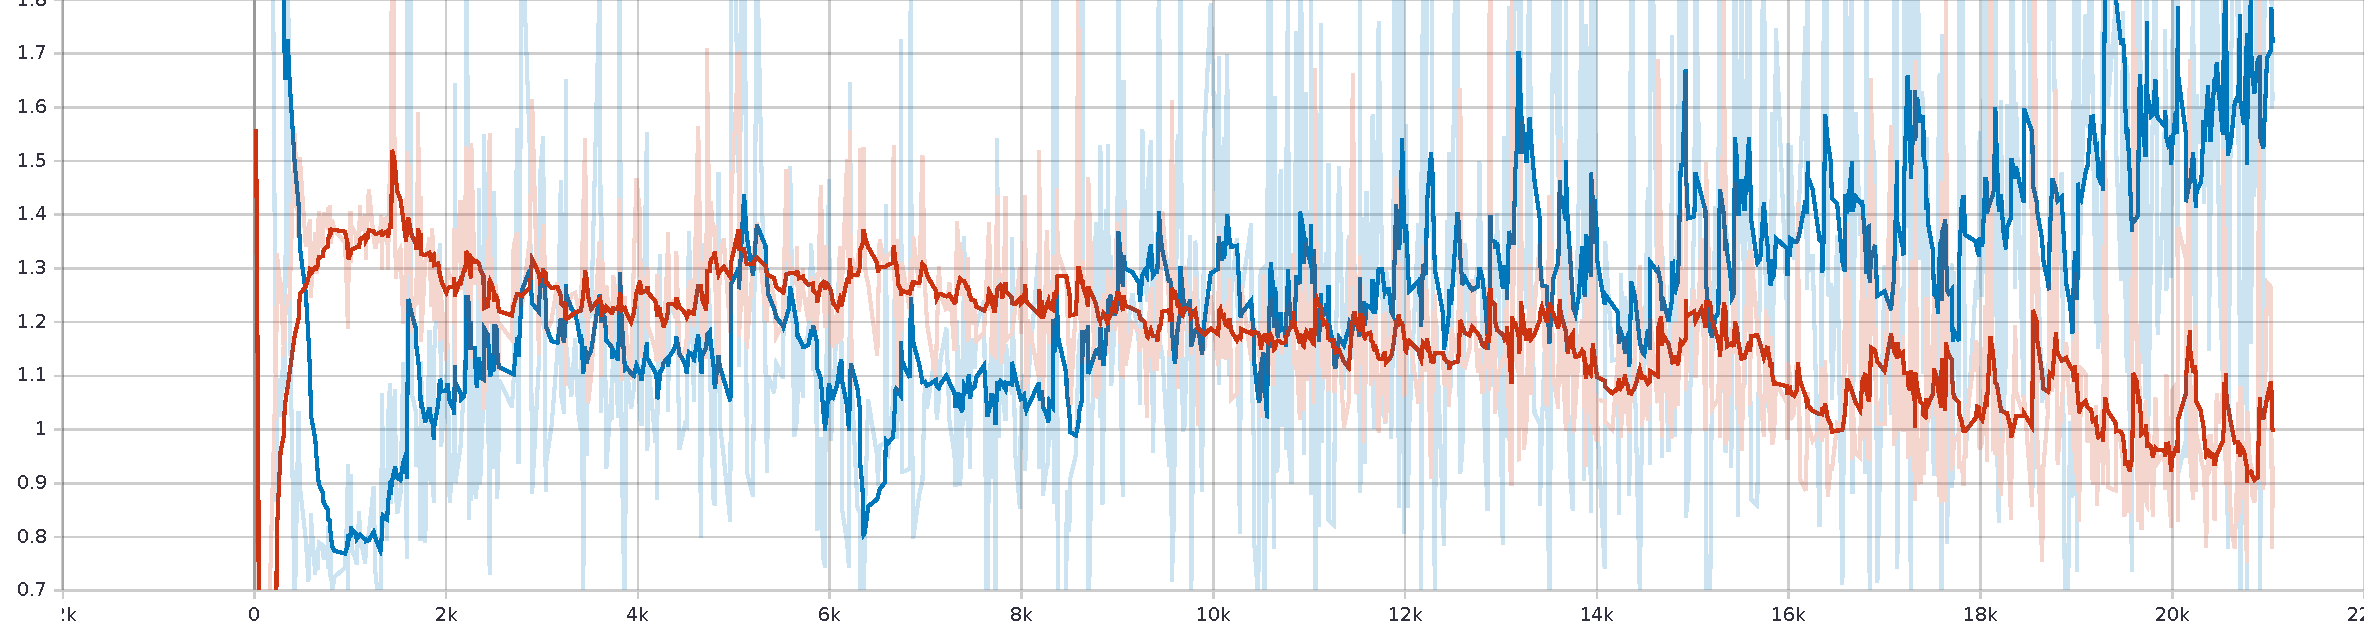
\includegraphics[width=1.5\linewidth]{SN(2)-DCGAN_loss.pdf}}
%\centerline{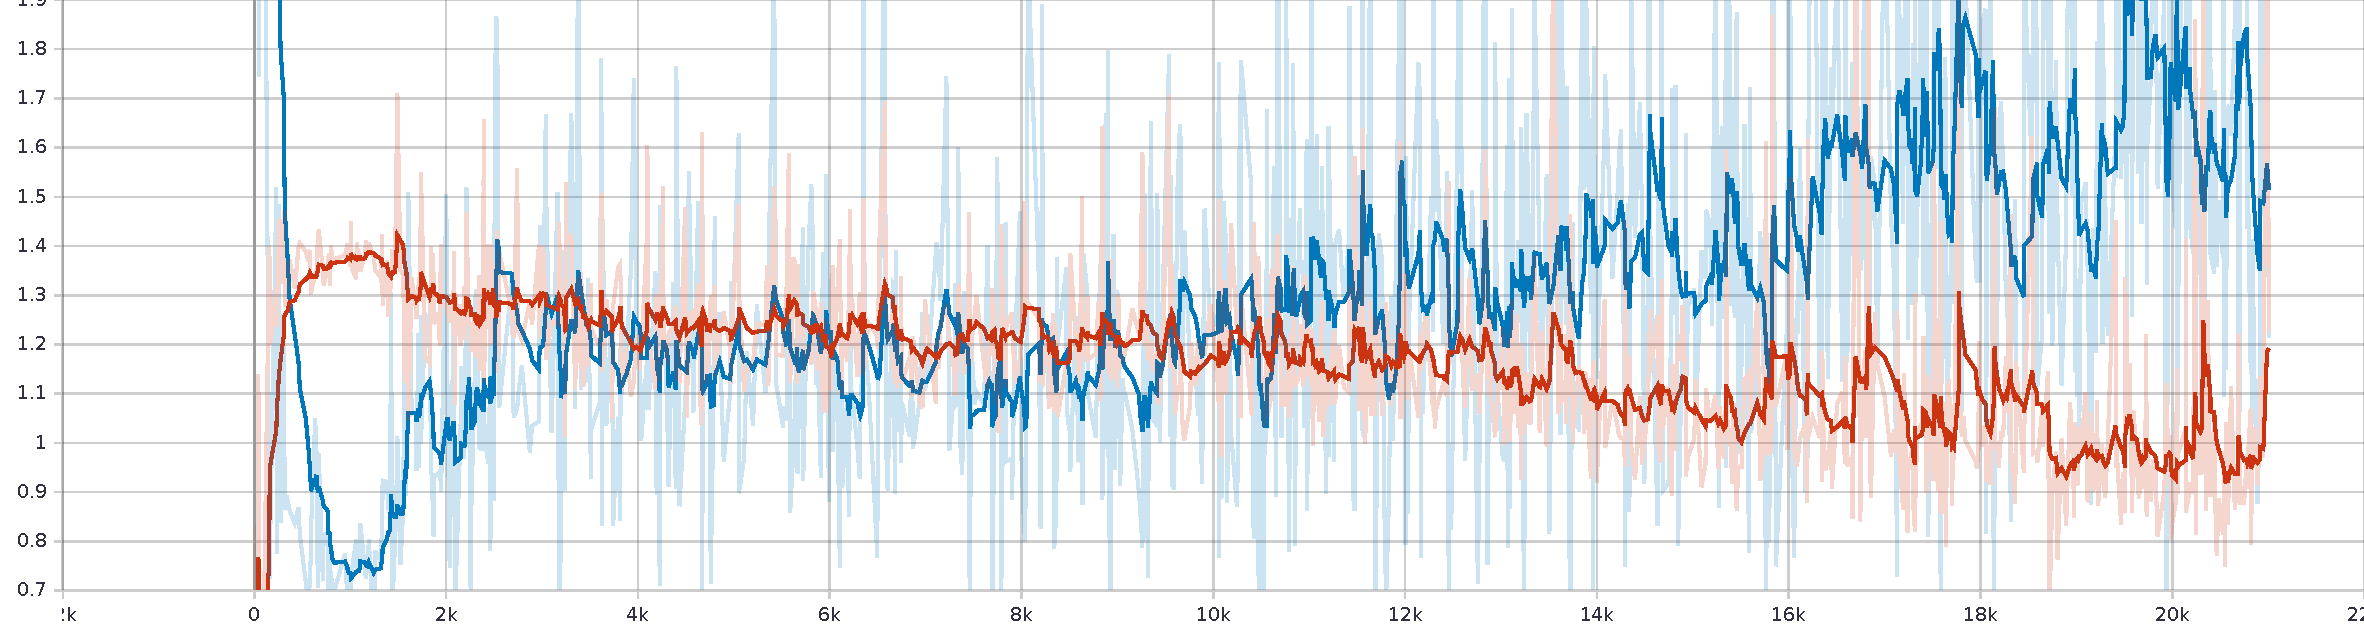
\includegraphics[width=1.5\linewidth]{SN(3)-DCGAN_loss.pdf}}

\newpage
\begin{thebibliography}{9}
	\bibitem{GAN-2014}
	Ian J. Goodfellow, Jean Pouget-Abadie, Mehdi Mirza, Bing Xu, David Warde-Farley, Sherjil Ozair, Aaron Courville, Yoshua Bengio. Generative Adversarial Nets. \textit{arXiv preprint arXiv:1406.2661}, 2014.
	
	\bibitem{Metrics-2018}
	Qiantong Xu, Gao Huang, Yang Yuan, Chuan Guo, Yu Sun, Felix Wu, Kilian Weinberger. An empirical study on evaluation metrics of generative adversarial networks. \textit{arXiv preprint arXiv:1806.07755}, 2018.
	
	\bibitem{DCGAN-2016}
	Alec Radford, Luke Metz, Soumith Chintala. Unsupervised Representation Learning with Deep Convolutional Generative Adversarial Networks. \textit{arXiv preprint arXiv:1511.06434}, 2016.
	
	\bibitem{SN-2018}
	Takeru Miyato, Toshiki Kataoka, Masanori Koyama, Yuichi Yoshida. Spectral Normalization for Generative Adversarial Networks. \textit{arXiv preprint arXiv:1802.05957}, 2018.
	
	\bibitem{WGAN-2017}
	Martin Arjovsky, Soumith Chintala, Léon Bottou. Wasserstein GAN. \textit{arXiv preprint arXiv:1701.07875}, 2017.
	
	\bibitem{GP-2017}
	Ishaan Gulrajani, Faruk Ahmed, Martin Arjovsky, Vincent Dumoulin, Aaron Courville. Improved Training of Wasserstein GANs. \textit{aXiv preprint arXiv:1704.00028}, 2017.
	
	\bibitem{IS-2016}
	Tim Salimans, Ian Goodfellow, Wojciech Zaremba, Vicki Cheung, Alec Radford, Xi Chen. Improved Techniques for Training GANs. \textit{arXiv preprint arXiv:1606.03498}, 2016.
	
	\bibitem{FID-2017}
	Martin Heusel, Hubert Ramsauer, Thomas Unterthiner, Bernard Nessler. GANs Trained by a Two Time-Scale Update Rule
	Converge to a Local Nash Equilibrium. \textit{NIPS}, 2017.
	
	\bibitem{CelebA-2015}
	Ziwei Liu, Ping Luo, Xiaogang Wang, Xiaoou Tang. Deep Learning Face Attributes in the Wild. \textit{Proceedings of International Conference on Computer Vision (ICCV)}, 2015.
	
	\bibitem{Inception-2014}
	Christian Szegedy, Wei Liu, Yangqing Jia, Pierre Sermanet, Scott Reed, Dragomir Anguelov, Dumitru Erhan, Vincent Vanhoucke, Andrew Rabinovich. Going Deeper with Convolutions. \textit{arXiv preprint arXiv:1409.4842}, 2014.
	
	\bibitem{ImageNet-2014}
	Olga Russakovsky, Jia Deng, Hao Su, Jonathan Krause, Sanjeev Satheesh, Sean Ma, Zhiheng Huang, Andrej Karpathy, Aditya Khosla, Michael Bernstein, Alexander C. Berg, Li Fei-Fei. ImageNet Large Scale Visual Recognition Challenge. \textit{arXiv preprint arXiv:1409.0575}, 2014.
	
	\bibitem{BN-2015}
	Sergey Ioffe, Christian Szegedy. Batch Normalization: Accelerating Deep Network Training by Reducing Internal Covariate Shift. \textit{arXiv preprint arXiv:1502.03167}, 2015.
	
	\bibitem{ReLU-2010}
	Vinod Nair, Geoffrey E. Hinton. Rectified linear units improve restricted boltzmann machines. \textit{ICML: Proceedings of the 27th International Conference on International Conference on Machine Learning}, 2010.
	
	\bibitem{Lipschitz-2017}
	Guo-Jun Qi. Loss-Sensitive Generative Adversarial Networks on Lipschitz Densities. \textit{arXiv preprint arXiv:1701.06264}, 2017.
	
	\bibitem{PyTorch-2019}
	Adam Paszke, Sam Gross, Francisco Massa, Adam Lerer, James Bradbury, Gregory Chanan, Trevor Killeen, Zeming Lin, Natalia Gimelshein, Luca Antiga, Alban Desmaison, Andreas Köpf, Edward Yang, Zach DeVito, Martin Raison, Alykhan Tejani, Sasank Chilamkurthy, Benoit Steiner, Lu Fang, Junjie Bai, Soumith Chintala. PyTorch: An Imperative Style, High-Performance Deep Learning Library. \textit{arXiv preprint arXiv:1912.01703}, 2019.
	
	\bibitem{Adam-2014}
	Diederik P. Kingma, Jimmy Ba. Adam: A Method for Stochastic Optimization. \textit{arXiv preprint arXiv:1412.6980}, 2014.
	
	\bibitem{CGAN-2014}
	Mehdi Mirza, Simon Osindero. Conditional Generative Adversarial Nets. \textit{arXiv preprint arXiv:1411.1784}, 2014.
	
	\bibitem{StyleGAN-2018}
	Tero Karras, Samuli Laine, Timo Aila. A Style-Based Generator Architecture for Generative Adversarial Networks. \textit{arXiv preprint arXiv:1812.04948}, 2018.
	
	\bibitem{StyleGAN2-2019}
	Tero Karras, Samuli Laine, Miika Aittala, Janne Hellsten, Jaakko Lehtinen, Timo Aila. Analyzing and Improving the Image Quality of StyleGAN. \textit{arXiv preprint arXiv:1912.04958}, 2019.
\end{thebibliography}

\end{document}